
\documentclass[twoside,11pt]{article}
%\documentclass[UTF8]{ctexart}
\usepackage[heading=true]{ctex}

\usepackage{listings}
\usepackage{color}

\definecolor{dkgreen}{rgb}{0,0.6,0}
\definecolor{gray}{rgb}{0.5,0.5,0.5}
\definecolor{mauve}{rgb}{0.58,0,0.82}

\lstset{frame=tb,
  language=Python,
  aboveskip=3mm,
  belowskip=3mm,
  showstringspaces=false,
  columns=flexible,
  basicstyle={\small\ttfamily},
  numbers=none,
  numberstyle=\tiny\color{gray},
  keywordstyle=\color{blue},
  commentstyle=\color{dkgreen},
  stringstyle=\color{mauve},
  breaklines=true,
  breakatwhitespace=true,
  tabsize=3
}

\usepackage{fancyhdr} % 页眉页脚
\usepackage{graphicx}
\usepackage{amsmath}
\usepackage[colorlinks=true, allcolors=blue]{hyperref}
%\usepackage[margin=1.5in]{geometry}

\oddsidemargin .25in    %   Note \oddsidemargin = \evensidemargin
\evensidemargin .25in
\marginparwidth 0.07 true in
%\marginparwidth 0.75 true in
%\topmargin 0 true pt           % Nominal distance from top of page to top of
%\topmargin 0.125in
\topmargin -0.1in
\addtolength{\headsep}{0.25in}
\textheight 8.5 true in       % Height of text (including footnotes & figures)
\textwidth 6.0 true in        % Width of text line.
\widowpenalty=10000
\clubpenalty=10000


\pagestyle{fancy}

%\firstpageno{1}

\title{Data\ Privacy\ Lab2}

\author{罗浩铭\ PB21030838}


\begin{document}

\fancyhf{} % 清除所有页眉页脚
\fancyfoot[C]{\thepage} % 设置右页脚为页码
\fancyhead[l]{\footnotesize USTC Data Privacy}
% 设置右页眉为章节标题 

\renewcommand{\headrulewidth}{0pt} % 去页眉线

\begin{center}
    \textbf{\LARGE{Data\ Privacy\ Lab2}}\\
    \vspace{0.1cm}
    \large{罗浩铭\ PB21030838}
\end{center}


% 实验报告要求:说明代码实现方法,简要给出实验结果说明,可以证明有效性即可

\section{代码实现}
\subsection{VFL-LR算法实现}
% (50`)基于 paillier 同态加密实现 VFL-LR 算法,保护训练中间变量,避免产生隐私泄露。
%  补全模型训练过程中的前向及反向传播的具体代码,记录 cancer 数据集在训练过程中的loss及acc变化。

\subsubsection{VFL-LR算法主逻辑}

VFL-LR算法主逻辑如图\ref{fig:VFL-LR}所示。

\begin{figure}[htbp]
    \centering
    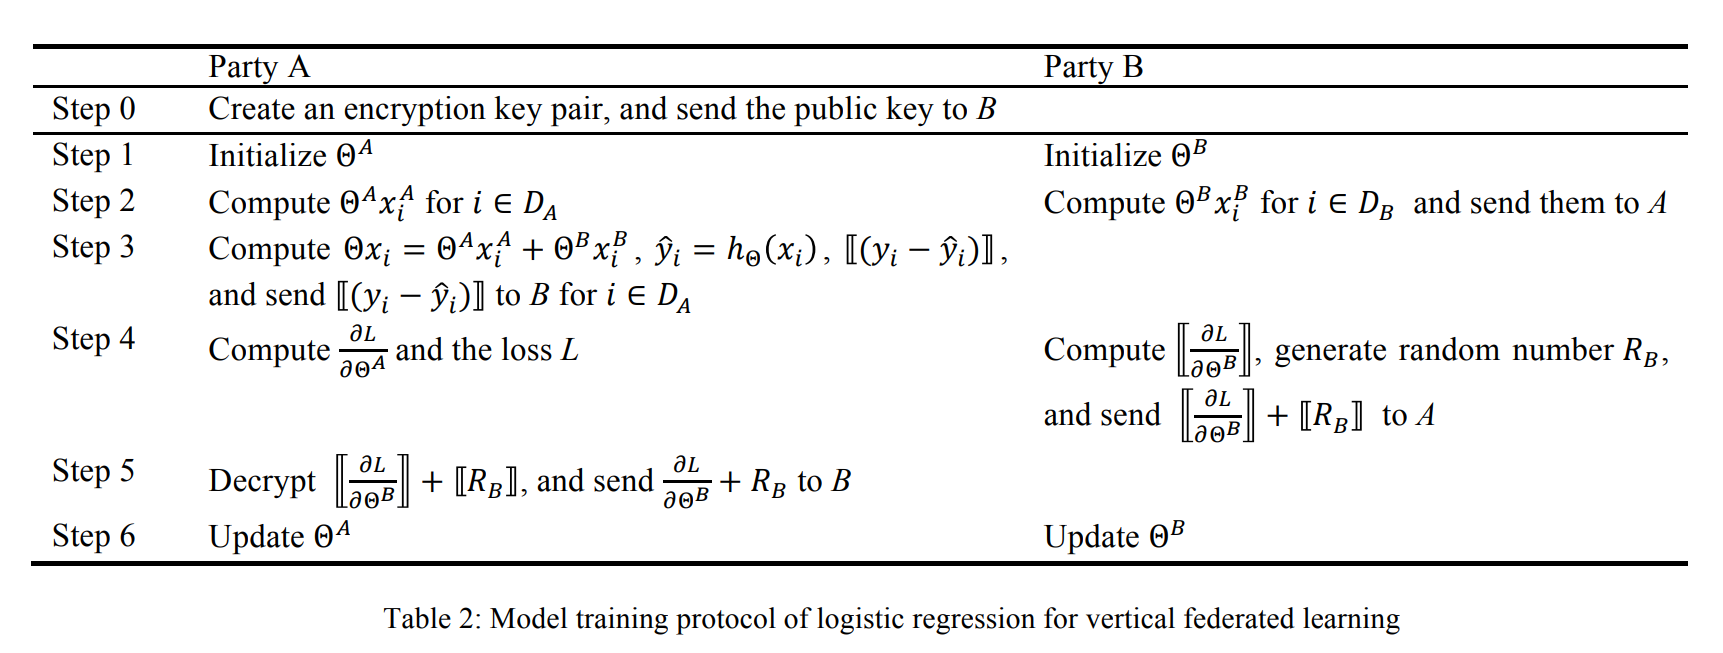
\includegraphics[width=0.8\textwidth]{pic/VFL-LR.png}
    \caption{VFL-LR算法主逻辑}
    \label{fig:VFL-LR}
\end{figure}

主逻辑的代码已经在附录中给出,下面对需要填空的部分进行重点讲解。

进入每个epoch中的batch循环之前,Party A和Party B会使用同一个密钥对数据进行shuffle,
从而使得每个batch中两边选择的样本下标一致,分别记为$D_A, D_B$。

主逻辑中第0步密钥生成与公钥分发、第1步模型初始化、第6步更新模型部分已实现。下面对第2步至第5步进行讲解。

\textbf{第二步:}

Party A计算$\Theta^A x_i^A$如下:
\begin{lstlisting}
    active_wx = np.dot(self.x_train[batch_idxes], self.params)  # (填空)计算A的wx
\end{lstlisting}

Party B计算$\Theta^B x_i^B$如下,并将结果发送给A:
\begin{lstlisting}
    passive_wx = np.dot(self.x_train[batch_idxes], self.params)  # (填空)计算B的wx
    self.messenger.send(passive_wx)
\end{lstlisting}

\textbf{第三步:}

Party A汇总$\Theta^A x_i^A$与$\Theta^B x_i^B$,计算出$y$的预测值如下:
\begin{lstlisting}
    full_wx = active_wx + passive_wx  # (填空)综合A、B的wx(纵向联邦综合结果的关键一步)
    y_hat = self.activation(full_wx)
\end{lstlisting}

由于纵向联邦学习中,Party A与Party B的数据中的列是不同的,
这里汇总两边结果时用的是加法实际上是相当于把两边的数据拼接起来,同时用拼接了两边参数的模型进行预测:
$$
    \Theta^A x_i^A + \Theta^B x_i^B =
    \begin{pmatrix}
        \Theta^A & \Theta^B
    \end{pmatrix}
    \begin{pmatrix}
        x_i^A \\
        x_i^B
    \end{pmatrix}
$$

再过个Sigmoid激活函数,就得到了$y$的预测值$\hat{y}=\mathrm{Sigmoid}(\Theta^A x_i^A + \Theta^B x_i^B)$

此后将预测值的误差(与真实值的残差)$y-\hat{y}$加密后传给Party B。
\begin{lstlisting}
    residue = self.y_train[batch_idxes] - y_hat
    residue = np.array([round(res, self.RESIDUE_PRECISION) for res in residue])

    enc_residue = self.cryptosystem.encrypt_vector(residue)  # (填空)对误差进行加密
    enc_residue = np.array(enc_residue)
    self.messenger.send(enc_residue)
\end{lstlisting}

其具体步骤为:计算残差,将浮点数精度舍入到指定精度,
调用Paillier加密函数 \\ \verb|self.cryptosystem.encrypt_vector| 将残差向量加密,并将加密后的残差向量$[[y-\hat{y}]]$发送给Party B。

\textbf{第四步:}

Party A直接利用残差$y-\hat{y}$反向传播计算梯度。
\begin{lstlisting}
    active_grad = self._gradient(residue, batch_idxes)
\end{lstlisting}

Party B收到加密的残差$[[ y-\hat{y} ]]$后,在密文空间进行同态计算得到密文空间中的梯度$[[\frac{\partial L}{\partial \Theta^B}]]$。

由于Paillier的同态性质,密文空间中的乘法对应明文中的加法,密文空间中的乘方对应明文中的数乘。
而反向传播计算梯度的过程中,只需用到加法和数乘,因此可以在密文空间中进行同态计算得到密文空间中的梯度。
(要注意的是:虽然同态空间内的“加法”是乘法,“数乘”是乘方,但人家phe库中的密文类已经帮你实现这一算符重载了,无需你自己关心这一细节)

此后,Party B将密文空间中的梯度$[[\frac{\partial L}{\partial \Theta^B}]]$加上一个随机数mask $[[R_B]]$后,发送给Party A。
\begin{lstlisting}
    enc_residue = self.messenger.recv()
    # print("enc_residue: ", enc_residue)
    enc_grad = self._gradient(enc_residue, batch_idxes)
    # print("enc_grad: ", enc_grad)
    enc_mask_grad, mask = self._mask_grad(enc_grad)
    self.messenger.send(enc_mask_grad)
\end{lstlisting}

加随机数mask的方法如下:
\begin{lstlisting}
    def _mask_grad(self, enc_grad):
        shape = enc_grad.shape
        mask = np.random.normal(0, 10.0, shape)  # 取随机数mask
        enc_mask = self.cryptosystem.encrypt_vector(mask)  # 加密mask
        enc_mask_grad = enc_grad + enc_mask  # 对密文进行同态加(这个加法被重载过,对应了Paillier密文的乘法)
        return enc_mask_grad, mask
\end{lstlisting}

首先我们取与原梯度相同shape且噪声足以基本盖过原梯度信息(这里取了标准差为10的随机正态分布)的随机数mask,
然后将mask加密,最后将加密后的mask与原梯度相加得到加上mask的梯度并返回(这里的加仍是同态空间的加,密文类重载的加法,也即实际上的乘法)。

\textbf{第五步:}
由于Paillier的同态性质,$[[\frac{\partial L}{\partial \Theta^B}]]+[[R_B]]=[[\frac{\partial L}{\partial \Theta^B}+R_B]]$,
而A持有私钥,因此将其解密可得$\frac{\partial L}{\partial \Theta^B}+R_B$,将其发送给B。
实现如下:
\begin{lstlisting}
    enc_passive_grad = self.messenger.recv()
    passive_grad = self.cryptosystem.decrypt_vector(enc_passive_grad)  # (填空)解密得到B的梯度与梯度之和
    self.messenger.send(passive_grad)
\end{lstlisting}

注意,上一步加上随机数就是为了让A在这一步无法得到B的梯度。

B收到$\frac{\partial L}{\partial \Theta^B}+R_B$后,将其减去随机数mask $R_B$得到$\frac{\partial L}{\partial \Theta^B}$,
\begin{lstlisting}
    mask_grad = self.messenger.recv()
    true_grad = self._unmask_grad(mask_grad, mask)
\end{lstlisting}

其中\verb |self._unmask_grad| 函数实现如下:
\begin{lstlisting}
    def _unmask_grad(self, mask_grad, mask):
        true_grad = mask_grad - mask  # 减去随机数mask得到梯度
        return true_grad
\end{lstlisting}

此时双方都得到了自己的参数梯度,可以进行第六步的参数更新了。

\subsubsection{Accuracy计算}
Accuracy的计算函数代码如下:
\begin{lstlisting}
    def _acc(self, y_true, y_hat):
        acc = np.mean(y_true == (y_hat >= 0.5))
        return acc
\end{lstlisting}

其计算逻辑为:
先将预测值$\hat{y}$中大于等于0.5的部分置为1,小于0.5的部分置为0,作为预测的label,
然后将其与与真实值$y$进行比较,得到一个布尔数组,表示每一位结果是否正确。
最后计算布尔数组的平均值,即为Accuracy。

为了运行效率,我们的实现中的每一步坚持使用向量化计算。

同时,要注意的是,布尔数组与0,1数组在绝大多数情况下等价,
布尔数组与0,1数组的比较、布尔数组的求平均值等操作中布尔数组的行为与0,1数组一致,也即在此函数内的每一步混用都是合法的。



\subsection{sacle函数的原理及作用}
% (20`)请说明代码中 scale 函数的原理及作用。



\subsection{随机数种子}
% (20`)当前代码在每个 epoch 开始时使用 epoch 值作为随机数种子,请说明含义,并实现另一种方式以达到相同的目的。

这是为了使得Party A\&B在每个epoch中使用相同的随机数,从而使得每次迭代中两边选择的样本下标一致,
从而可以将两边得到的label直接相加即可得到最终结果,也使得此结果可对正确下标的输入样本进行反向传播求导。

我们可以使用其他方式来实现相同的目的,比如:
每一个epoch中,B生成随机数种子,将其用公钥加密后发送给A,A用私钥解密后得到该种子,此后该epoch内两边都使用此种子生成随机数。

\section{实验结果}
我们使用了默认参数进行实验。

实验测得的各个epoch下的loss和accuracy值图像如图\ref{fig:loss}和图\ref{fig:acc}所示。

\begin{figure}[htbp]
    \centering
    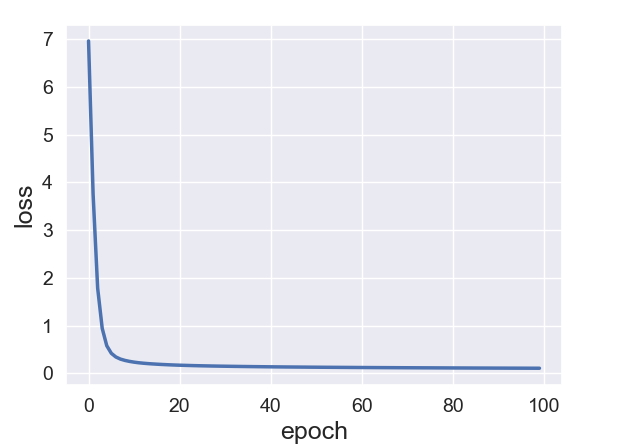
\includegraphics[width=0.8\textwidth]{pic/loss-plot.png}
    \caption{各epoch下的loss值图像}
    \label{fig:loss}
\end{figure}

\begin{figure}[htbp]
    \centering
    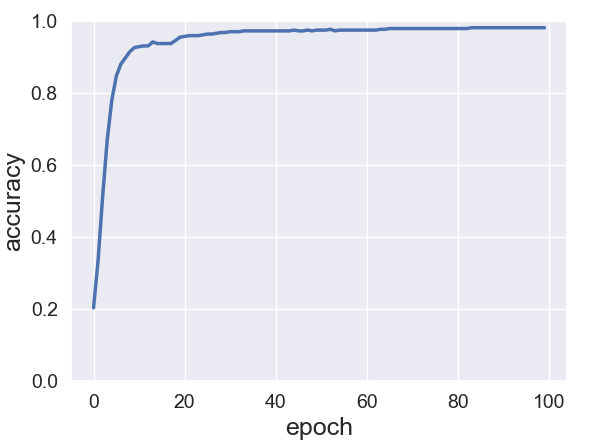
\includegraphics[width=0.8\textwidth]{pic/accuracy-plot.png}
    \caption{各epoch下的accuracy值图像}
    \label{fig:acc}
\end{figure}

经过100个epoch的训练,最终得到的准确率为0.980,loss值为0.105。这样的准确率证明了我们的实现方案的有效性。

在本人的搭载AMD Ryzen 7 4800H CPU、内存16GB的笔记本电脑上,100个epoch的训练时间约为20分钟,每个epoch约需12s来训练。

其中Active端进程输出如图\ref{fig:active}所示,Passive端进程输出如图\ref{fig:passive}所示。

\begin{figure}[htbp]
    \centering
    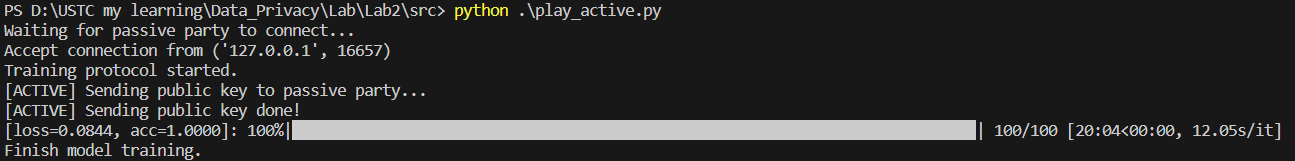
\includegraphics[width=0.8\textwidth]{pic/active-output.png}
    \caption{Active端进程输出}
    \label{fig:active}
\end{figure}

\begin{figure}[htbp]
    \centering
    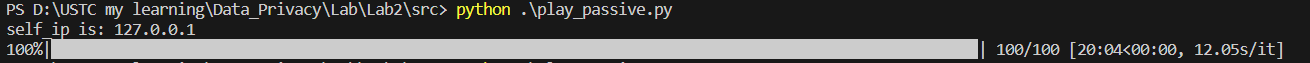
\includegraphics[width=0.8\textwidth]{pic/passive-output.png}
    \caption{Passive端进程输出}
    \label{fig:passive}
\end{figure}


\section{实验分析及开放题}
% (10`)开放题:试分析VFL-LR训练流程中潜在的隐私泄露风险,并简要说明可能的保护方式

$\Theta^B x_i^B$的label泄露

$\frac{\partial L}{\partial \Theta^B}+R_B$

\appendix
\section*{附录}

\section{Party A (Active Party)对一个batch进行处理的具体实现}

\begin{lstlisting}
total_loss = 0.0
total_acc = 0.0

for batch in range(n_batches):
    # Choose batch indexes
    start = batch * bs
    end = len(all_idxes) if batch == n_batches - 1 else (batch + 1) * bs
    batch_idxes = all_idxes[start:end]

    # Q1. Active party calculates y_hat
    # -----------------------------------------------------------------
    # self.params: (n_features, )
    # self.x_train[batch_idxes]: (batch_size, n_features)
    active_wx = np.dot(self.x_train[batch_idxes], self.params)  # (填空)计算A的wx
    passive_wx = self.messenger.recv()
    full_wx = active_wx + passive_wx  # (填空)综合A、B的wx(纵向联邦综合结果的关键一步)
    y_hat = self.activation(full_wx)
    # -----------------------------------------------------------------

    loss = self._loss(self.y_train[batch_idxes], y_hat)
    acc = self._acc(self.y_train[batch_idxes], y_hat)
    tbar.set_description(f"[loss={loss:.4f}, acc={acc:.4f}]")
    total_acc += acc * len(batch_idxes)
    total_loss += loss * len(batch_idxes)

    residue = self.y_train[batch_idxes] - y_hat
    residue = np.array([round(res, self.RESIDUE_PRECISION) for res in residue])

    # Q2. Active party helps passive party to calculate gradient
    # -----------------------------------------------------------------
    enc_residue = self.cryptosystem.encrypt_vector(residue)  # (填空)对误差进行加密
    enc_residue = np.array(enc_residue)
    self.messenger.send(enc_residue)

    enc_passive_grad = self.messenger.recv()
    passive_grad = self.cryptosystem.decrypt_vector(enc_passive_grad)  # (填空)解密得到B的梯度与梯度之和
    self.messenger.send(passive_grad)
    # -----------------------------------------------------------------

    # Active party calculates its own gradient and update model
    active_grad = self._gradient(residue, batch_idxes)
    self._gradient_descent(self.params, active_grad)
\end{lstlisting}

\section{Party B (Passive Party)对一个batch进行处理的具体实现}

\begin{lstlisting}
for batch in range(n_batches):
    # Choose batch indexes
    start = batch * bs
    end = len(all_idxes) if batch == n_batches - 1 else (batch + 1) * bs
    batch_idxes = all_idxes[start:end]

    # Q1. Calculate wx and send it to active party
    # -----------------------------------------------------------------
    passive_wx = np.dot(self.x_train[batch_idxes], self.params)  # (填空)计算B的预测值
    self.messenger.send(passive_wx)
    # -----------------------------------------------------------------

    # Q2. Receive encrypted residue and calculate masked encrypted gradients
    # -----------------------------------------------------------------
    enc_residue = self.messenger.recv()
    # print("enc_residue: ", enc_residue)
    enc_grad = self._gradient(enc_residue, batch_idxes)
    # print("enc_grad: ", enc_grad)
    enc_mask_grad, mask = self._mask_grad(enc_grad)
    self.messenger.send(enc_mask_grad)
    # Receive decrypted masked gradient and update model
    mask_grad = self.messenger.recv()
    true_grad = self._unmask_grad(mask_grad, mask)
    # -----------------------------------------------------------------

    self._gradient_descent(self.params, true_grad)
\end{lstlisting}

\end{document}
